% \documentclass{report}
% 
% \usepackage{fancyhdr}
\usepackage{fourier-orns}
\usepackage{hyperref}%% To refrence links / jumps
\usepackage{chngcntr} %% For some extra counters numberings
\usepackage[a4paper, right = 0.5in, left = 0.5in,top = 1in , bottom = 1in]{geometry}
\usepackage{etoolbox} %% Provides like a language for advanced customization
\usepackage{datetime} %% For dates of course
\usepackage{lastpage} %% provides pages numbers
\usepackage[sc]{titlesec} %% modify titles
\usepackage{enumerate}
\usepackage{cancel}
\usepackage{tikzsymbols}
\usepackage[dvipsnames]{xcolor}
\usepackage{import}
\usepackage{pdfpages} %% include other pdfs
\usepackage{transparent} %% Transparency
\usepackage{xcolor}  %% Colors
\usepackage[many]{tcolorbox}
\usepackage[framemethod=TikZ]{mdframed}
\usepackage{amsmath,amsfonts,amsthm,amssymb,mathtools}
\usepackage{tikz}
\usepackage{bookmark}
\usepackage{graphicx}
\usepackage{mathpazo}

\usepackage{fontawesome5}

\linespread{1.5}


\titleformat{\chapter}[display]   
{\fontfamily{ppl}\selectfont\huge\color{YellowOrange!80!orange}} % Font style and size 
{\raggedleft\color{purple}\fontsize{70}{0pt}\selectfont\thechapter}   
{-1.5cm}    			                          % Space between the chapter number and title
{
	\begin{tikzpicture}[overlay]
		\node[anchor = west,yshift = 0.2cm,xshift = -1cm] {\fontsize{90}{20} $\int_{}^{} $};
		\node[yshift = 4cm, xshift = 17cm]   {\includegraphics[width = 4cm]{preview0}};
	\end{tikzpicture}
\hspace{1cm}\Huge\raggedright\MakeUppercase}

\titleformat{\section}[block]
{
\fontfamily{ppl}\selectfont\huge\color{YellowOrange!80!orange}
}
{
\color{purple}\fontsize{20}{0pt}\selectfont\thesection 
}
{0cm}
{
	\begin{tikzpicture}[overlay]
		\node[anchor = west,yshift = 0.2cm,xshift = -0.4cm, circle = 1pt] {};
	\end{tikzpicture}
}

\titlespacing*{\section}{0pt}{0.7cm}{1.5cm}


\newcommand{\divider}
{
	\begin{center}
	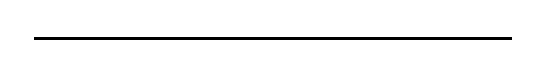
\begin{tikzpicture}
		\draw[thick, black] (0.25*\textwidth, 0) -- (0.75*\textwidth, 0);
		\node[rotate = 360 - 90, xshift = -0.6pt, yshift = 1pt] at (0.25*\textwidth,0){\decotwo};
		\node[rotate = 90, xshift = -0.6pt, yshift = 1pt] at (0.75*\textwidth,0){\decotwo};
	\end{tikzpicture}
	\end{center}
}

\pagestyle{fancy}

\newcommand{\lecday}[1][]
{
    \def\datee{#1}
    \fancyhead[L]{\datee}
}



\newcommand{\signature}
{
	\begin{tikzpicture}[remember picture,overlay]
		\node[fill = YellowOrange!20!white] at ([yshift = 1cm, xshift = -3cm]current page.south east) {\fontsize{10pt}{0pt}{\itshape Kara.$\mathcal{A}$}};
	\end{tikzpicture}
}

\AddToHook{shipout/background}{
  \begin{tikzpicture}[remember picture, overlay]
	  \node[] at ([yshift = 1.5cm,xshift = \textwidth /2 + 0.9cm]current page.south west) {\includegraphics[width = 0.5cm]{preview3}};
	  \node[] at ([yshift = 1.5cm,xshift = - \textwidth /2 - 0.9cm]current page.south east) {\includegraphics[width = 0.5cm]{preview4}};
  \end{tikzpicture}
}



\newtcolorbox[auto counter, number within = section]{remark}[1][]
{
       		title = Remark #1,
		enhanced,
		boxrule = 0pt,
		colback = white,
		breakable,
		arc = 4pt,
		colbacktitle = cyan,
		colback = cyan!5!white,
		segmentation style =
		{
			solid,cyan,thick,
		},
		attach boxed title to top left =
		{
			xshift = 0cm,
		},
		boxed title style =
		{
			boxrule = 0pt,
			sharp corners,
			drop fuzzy shadow = {cyan},
		},
		drop fuzzy shadow = {cyan!80!black},
}

\newtcolorbox[auto counter, number within = section]{theorem}[1][]
{                                      
		title = Theorem \thetcbcounter : #1,
		enhanced, 
		boxrule = 0pt,
		colback = white,
		breakable,
		arc = 4pt,
		colbacktitle = purple,
		colback = purple!5!white,
		segmentation style = 
		{
			solid, purple,thick,
		},
		attach boxed title to top left = 
		{
			xshift = 0cm, 
		},
		boxed title style = 
		{
			boxrule = 0pt,
			sharp corners,
			drop fuzzy shadow = {purple},
		},
		drop fuzzy shadow = {purple!80!black},
}

\newtcolorbox[auto counter, number within = section]{definition}[1][]
{                                      
		title = Definition \thetcbcounter : #1,
		enhanced, 
		boxrule = 0pt,
		colback = white,
		arc = 4pt,
		breakable,
		colbacktitle = YellowOrange!80!black,
		segmentation style = 
		{
			solid, YellowOrange,thick,
		},
		attach boxed title to top left = 
		{
			xshift = 0cm, 
		},
		colback = YellowOrange!5!white,
		boxed title style = 
		{
			boxrule = 0pt,
			sharp corners,
			drop fuzzy shadow = {YellowOrange!80!orange},
		},
		drop fuzzy shadow = {YellowOrange!80!black},
}

\newtcolorbox[auto counter, number within = section]{corollary}[1][]
{                                      
		title = corollary \thetcbcounter : #1,
		enhanced, 
		boxrule = 0pt,
		colback = white,
		arc = 4pt,
		breakable,
		colbacktitle = YellowOrange!80!black,
		segmentation style = 
		{
			solid, YellowOrange,thick,
		},
		attach boxed title to top left = 
		{
			xshift = 0cm, 
		},
		colback = YellowOrange!5!white,
		boxed title style = 
		{
			boxrule = 0pt,
			sharp corners,
			drop fuzzy shadow = {YellowOrange!80!orange},
		},
		drop fuzzy shadow = {YellowOrange!80!black},
}


\newtcolorbox{example}[1][]
{                                      
		title = Example,
		enhanced, 
		boxrule = 0pt,
		colback = white,
		arc = 4pt,
		segmentation style = 
		{
			solid, SpringGreen,thick,
		},
		breakable,
		colback = SpringGreen!5!white,
		colbacktitle = SpringGreen!80!black,
		attach boxed title to top left = 
		{
			xshift = 0cm, 
		},
		boxed title style = 
		{
			boxrule = 0pt,
			sharp corners,
			drop fuzzy shadow = {SpringGreen!80!orange},
		},
		drop fuzzy shadow = {SpringGreen!80!black},
}


\newcommand{\integral}[4]{\int\limits_{#1}^{#2} #4 d#3}
\newcommand{\limit}[3]{\lim\limits_{#1 \rightarrow #2} #3}
\newcommand{\strone}[2]{\left[ \begin{gathered}#1\\ #2\end{gathered} \right] }
\newcommand{\strtwo}[2]{\left\{ \begin{gathered}#1\\ #2\end{gathered} \right\} }
\newcommand{\strthree}[2]{\left\lfloor \begin{gathered}#1\\ #2\end{gathered} \right\rfloor }


\newcommand{\startbf}[1]{\text{\bfseries{#1}}}
\newcommand{\sett}[1]{\left\{ #1 \right\}}
\newcommand{\thesis}[1]{\left( #1 \right)}
\newcommand{\brkt}[1]{\left[ #1 \right]}
\newcommand{\floor}[1]{\left\lfloor #1 \right\rfloor}


\DeclareMathOperator{\img}{im} % Image
\DeclareMathOperator{\Img}{Im} % Image
\DeclareMathOperator{\coker}{coker} % Cokernel
\DeclareMathOperator{\Coker}{Coker} % Cokernel
\DeclareMathOperator{\Ker}{Ker} % Kernel
\DeclareMathOperator{\rank}{rank}
\DeclareMathOperator{\Spec}{Spec} % spectrum
\DeclareMathOperator{\Tr}{Tr} % trace
\DeclareMathOperator{\pr}{pr} % projection
\DeclareMathOperator{\ext}{ext} % extension
\DeclareMathOperator{\pred}{pred} % predecessor
\DeclareMathOperator{\dom}{dom} % domain
\DeclareMathOperator{\ran}{ran} % range
\DeclareMathOperator{\Hom}{Hom} % homomorphism
\DeclareMathOperator{\Mor}{Mor} % morphisms
\DeclareMathOperator{\End}{End} % endomorphism


\newcommand{\lm}{\ensuremath{\lambda}}
\newcommand{\eps}{\ensuremath{\epsilon}}
\newcommand{\veps}{\ensuremath{\varepsilon}}
\newcommand{\al}{\ensuremath{\alpha}}
\newcommand{\bb}{\ensuremath{\beta}}
\newcommand{\cc}{\ensuremath{\gamma}}
\newcommand{\dd}{\ensuremath{\delta}}
\newcommand{\DD}{\ensuremath{\Delta}}
\newcommand{\ff}{\ensuremath{\phi}}
\newcommand{\FF}{\ensuremath{\varphi}}

\newcommand{\RR}{\mathbb{R}}
\newcommand{\RO}{\mathcal{R}}
\newcommand{\EE}{\mathbb{E}}
\newcommand{\CC}{\mathbb{C}}
\newcommand{\RW}{\mathbb{R}^2}
\newcommand{\RT}{\mathbb{R}^3}
\newcommand{\RN}{\mathbb{R}^n}
\newcommand{\DS}{\mathcal{D}}

\newcommand{\KK}{\mathbb{K}}
\newcommand{\KW}{\mathbb{K}^2}
\newcommand{\KT}{\mathbb{K}^3}
\newcommand{\KN}{\mathbb{K}^n}

\newcommand{\NN}{\mathbb{N}}

\newcommand{\PS}{\mathcal{P}}
\newcommand{\AS}{\mathcal{E}}
\newcommand{\FS}{\mathcal{F}}
\newcommand{\LS}{\mathcal{L}}
\newcommand{\MS}{\mathcal{M}}


















\lecday[2025-04-10]

% \begin{document}
\begin{theorem}[]
	Let $E $ be a Banach space. Then every general series
	$\sum_{i \in  I}^{} x_{i} $ of $E $ which satisfies Cauchy 
	criterion is summable.
\end{theorem}
\begin{proof}
Let $\sum_{i \in  I}^{} x_{i} $ be a general series $E $ which satisfies
the Cauchy criterion, Then for all $n \in \NN $, $\exists  I_{n} \subset I $,
with $I_{n} $  finite, such that $\forall J $ a finite subset of
$I $, with $J \cap I_{n} = \emptyset  $, we have, 
\[
\| \sum_{i \in J}^{} x_{i} \|  < \frac{1}{n} 
\]
Let us define for all $n \in \NN $, 
\[
S_{n} := \sum_{i \in  I_1 \cup I_2 \cup \hdots \cup I_{n}}^{}  x_{i} 
\left( \in  E \right)
\]
Clearly, $(S_{n}) _{n \in \NN} $  is a sequence of $E$.

we have for any $p,q \in \NN $, with $p > q $, 
\begin{align*}
\| S_{p} - S_{q} \|  = 
\| \sum_{i \in I_1 \cup \hdots \cup  I_{p}}^{} x_{i} - 
\sum_{i \in I_1 \cup  \hdots  \cup  I_{q}}^{} x_{i} \|  &=
\| \sum_{i \in 
\underbrace{
( I_1 \cup \hdots  I_{p}) \backslash  (I_1 \cup  \hdots  \cup I_{q}) 
}_{ \text{ finite, disjoint with $I_{q} $ } } 
}^{}  
x_{i}\|  <  \frac{1}{q}
\end{align*}
Hence $\lim_{p,q \to \infty} \| S_{p} - S_{q} \| = 0 $, implying
that $(S_{n}) _{n \in \NN} $ is Cauchy since $E $ is Banach then 
$\left( S_{n} \right)_{n \in \NN} $ is convergent. Let
$S := \lim_{n \to \infty }  S_{n} \in E$, and let us show that the general
series $\sum_{i \in I}^{} x_{i} $  is summable with sum $S$ 
$\forall  \veps  > 0, \exists I_{\veps  }\subset I, \text{ with } 
I_{\veps } \text{ finite }, \forall  J \subset I, \text{ J finite }$
\[
I_{\veps }\subset  J \implies 
\| \sum_{i \in J}^{} x_{i} - S \|  <  \veps 
\]

Let $\veps  > 0 $ arbitrary then since $S_{n} \rightarrow S $ 
in $E $ and 
$\frac{1}{n} \rightarrow 0 $  as $n \rightarrow \infty  $  in $\RR  $, 
then $\exists  n_0  \in \NN$ , such that, 
\[
\| S_{n_0} - S \|  < \frac{\veps }{2} \text{ and } 
\frac{1}{n_0} <  \frac{\veps }{2}
\]
take $I_{\veps } = I_1 \cup  \hdots  \cup  I_{n_0}$, 
For any subset $J $ of $I$ whixh is finite 
and contains $I_{\veps } $, we have, 
\begin{align*}
\| \sum_{i \in J}^{} x_{i} - S  \|  = 
\| \sum_{i \in  I_1 \cup \hdots \cup  I_{n_0}}^{}  x_{i} + 
\sum_{i \in  J \backslash 
(I_1 \cup  \hdots \cup  I_{n_0}) }^{} x_{i} - S\|   
&= \| S_{n_0} - S + \sum_{i \in J \backslash 
(I_1 \cup  \hdots  \cup  I_{n_0}) }^{} x_{i}  \|  \\
& \leq 
\underbrace{
\| S_{n_0} - S \|   
}_{ < \veps/2} 
+
\| \sum_{i \in  J \backslash ( I_1 \cup  \hdots  \cup  
I_{n_0}) }^{} x_{i}  \|   \\
& <  \veps 
\end{align*}
Thus $\sum_{i \in I}^{} x_{i} $  is 
summable with sum $S $, hence the proof is complete.
\end{proof}
\divider
	\begin{center}
		Let $E $ be N.V.S prove that if a general 
		series of $E $ is summable 
		then it satisfies the Cauchy criterion
	\end{center}
\divider
\begin{definition}[]
Let $E $ be a N.V.S and $\sum_{ i \in  I}^{} x_{i} $  
be a general series of $E $, We say that $\sum_{i \in  I}^{} x_{i} $  
is normally summable if the real general 
series $\sum_{ i \in I}^{} \| x_{i} \|  $  
is summable.
\end{definition}
\begin{theorem}[]
Let $E $ be a Banach Space and $\sum_{i \in  I}^{} x_{i}  $  
be a general series, if $\sum_{i \in  I}^{} x_{i} $  is 
normally summable then its summable and we have 
\[
\| \sum_{i \in  I}^{} x_{i} \|  \leq 
\sum_{i \in  I}^{}  
\| x_{i} \| 
\]
\end{theorem}
\begin{proof}
Suppose that $\sum_{i \in I}^{} x_{i} $  is normally summable,
that is, the real general series $\sum_{i \in  I}^{} 
\| x_{i} \| $  is summable, Thus $\sum_{ i \in  I}^{} 
\| x_{i} \| $ satisfies the Cauchy criterion (see Previous exercise).

It follows that $\sum_{i \in  I}^{} x_{i} $  also satisfies the Cauchy
criterion 
$
\forall  \veps  > 0, \exists  I_{\veps }\subset I \text{ finite } , 
\forall  J \subset , \text{ J finite }, J \cap I_{\veps } = \emptyset  
$
\[
\implies  
\sum_{i \in  J}^{}  \|  x_{i} \|  <  \veps  
\implies 
\| \sum_{i \in  J}^{} x_{i}  \|  <  \veps 
\]
Thus according to the previous theorem, 
The general series $\sum_{i \in  I}^{} x_{i} $  
is summable as required.


Now, let us prove the inequality of the theorem, 
Let $S := \sum_{i \in  I}^{} x_{i}  $  
and $S' := \sum_{i \in  I}^{} \| x_{i} \| \in  \RR  $, 
we have to show that $\| S \|  \leq  S' $,  
For all $\veps  > 0 $, there exist $I_{ \veps  } \subset I $, 
with $I_{\veps } $ finite such that $\forall  J \subset I $, such that 
$J $ finite, 
\[
I_{\veps } \subset J \implies 
\| \sum_{i \in  J}^{}  x_{i} - S\|  <  \veps 
\]
Similarly, for all $\veps > 0 $, there exist $I_{\veps }' \subset I $,
with $I_{\veps }' $  finite, such that $\forall  J \subset I $, with 
$J $ finite, with $J $ finite, 
\[
I_{\veps }' \subset J \implies 
\| \sum_{i \in  J}^{} \|  x_{i} \| - S' \|  <  \veps 
\]
For $\veps > 0 $, by taking 
$J = I_{\veps } \cup  I_{\veps }' $, we have 
\begin{align*}
	\| \sum_{i \in  J}^{} x_{i} - S \|  &<  \veps 
\\
	\| \sum_{i \in  J}^{} \| x_{i} \| - S' \|  &<   \veps 
\end{align*}
Hence, using the above inequalitys, we have, 
\begin{align*}
	\| S \|  &= 
\| S - \sum_{i \in  J}^{}  x_{i} + \sum_{i \in  J}^{} x_{i}  \|  
		 \\
		 & \leq 
		 \underbrace{
		 \| S - \sum_{i \in  J}^{} x_{i} \|  + 
		 }_{ <  \veps  } 
		 \underbrace{
		 \sum_{i \in  J}^{}  \| x_{i} \|  
		 }_{<  S' + \veps } \\ 
		 & <  S' + 2\veps 
\end{align*}
Thus $ \| S \|  <  S' + 2 \veps  $  for all $ \veps  > 0 $, by taking 
$ \veps  \rightarrow 0^{+} $  gives $ \|  S \|  \leq  S' $, as required.
this completes the proof.
\end{proof}

The following theorem shows that every generla series of 
a N.V.S, can always be reduced to an ordinary series i.e 
$I = \NN $.

\begin{theorem}[]
	Let $E $ be a N.V.S and 
	$\sum_{i \in  I}^{ } x_{i}$, be a general 
	series of $E $, Suppose that $\sum_{i \in  I}^{} 
	x_{i}$ is summable. then the set 
	\[
	I' := 
	\left\{ i \in  I: x_{i} \neq 0_{E} \right\}
	\]
	is at most countable. In addition, the general series $\sum_{
	i \in  I'}^{} x_{i} $ is summable and we have 
	\[
	\sum_{i \in   I'}^{} x_{i} = 
	\sum_{i  \in I}^{}  x_{i}
	\]
\end{theorem}
\begin{proof}
for all $n \in  \NN $, put 
\[
I_{n}' := 
\left\{ i \in  I: 
\| x_{i} \|  >  \frac{1}{n}\right\}
\]
So, we have that 
\begin{align*}
	\bigcup_{n \in  \NN}^{}  I_{n}' &=
	\left\{ i \in  I: \exists n \in  \NN 
	\text{ such that }  \| x_{i} \| > \frac{1}{n} \right\} \\
					&= 
					\left\{ i \in  I: 
				x_{i} \neq  0_{E}\right\} =
				I'
\end{align*}
\[
I = \bigcup_{n \in  \NN}^{} I_{n}'
\]
Next, let us prove that $I_{n}' $ is finite for every $n \in \NN $. 
So let $n \in \NN $ , since $\sum_{i \in  I}^{}  x_{i}$ 
is assumed to be summable then it satisfies the Cauchy criterion,
So $\exists  I_{n} \subset I $, with $I_{n} $ finite, such that 
$\forall J \subset I $, with $J$ finite, 
\[
J \cap I_{n} = \emptyset \implies 
\| \sum_{i \in  J}^{} x_{i} \|  
<  \frac{1}{n}
\]
\begin{center}
(Cauchy criterion for $\veps = \frac{1}{n} $) 
\end{center}
In Particular, for every $j \in  I $, we have 
for $J = \left\{ j \right\}$,
\[
\forall j \in  I, \left\{ j \right\} \cap I_{n} =\emptyset 
\implies \| x_{j} \|  <  \frac{1}{n}
\]
Equivalently, 
\begin{align*}
\forall j \in  I, 
j \notin I_{n} & \implies 
\| x_{j} \|  <  \frac{1}{n} \\
	       & \implies 
	       j \notin  I_{n}' \\
	    \forall  j \in  I, 
	    j \notin I_{n} \implies 
	    j \notin  I_{n} '
\end{align*}
By the contrapositive we have, 
\begin{align*}
	\forall  j \in  I, j \in I_{n}' \implies 
	j \in  I_{n}
\end{align*}
Thus, 
\[
I_{n}' \subset I_{n}
\]
Since $I_{n} $ is finite, we derive that 
$I_{n}' $ is finite.

Consequently according to the above, 
$I' $  is a countable union of finite sets,
implying that $I' $ is at most countable, 
as required.

Now, let us prove the second part of the theorem,
 set $S := \sum_{i \in  I}^{} x_{i} $  
 then 
 $
 \forall  \veps  >  0, \exists  I_{\veps } \subset I, \text{ with } 
 I_{\veps }   \text{ finite }, \forall J \subset I, 
 \text{ with  J finite, we have, } $ 
 \[
 I_{\veps } \subset J \implies 
 \| \sum_{i \in  J}^{} x_{i} - S \|  <  \veps 
 \]
 Let $\veps  > 0 $ be arbitrary, by putting $I_{\veps }' = 
 I_{\veps } \cap I'$, which is finite since $I_{\veps } $ is finite and 
 $\subset I' $, we have for any finite subset $J' $ of $I' $, containing
 $I_{\veps }' $, 
 \begin{align*}
	 \sum_{i \in  J'}^{} x_{i} &= 
 \sum_{i \in  J' \cup  I_{\veps }'}^{}  x_{i} 
 \quad \quad 
 \text{ since $I_{\veps }' \subset J' $ }   \\
				   &= 
				\sum_{i \in  
				(J' \cup  I_{\veps }) \cap 
			I'}^{}  
		x_{i}  \\
				   &= \sum_{
				   i \in  J' \cup  I_{\veps }'}^{}  
				   x_{i}
 \end{align*}
 But since $J' \cup  I_{\veps } $  
 is finite and contains $I_{\veps } $  it fololws that 
 \[
 \|  \sum_{i \in  J'}^{} x_{i} - S \|  = 
 \| \sum_{i \in J' \cup  I_{\veps }}^{} x_{i} -S \|  <  \veps 
 \]
 This concludes that 
 the general series 
 $\sum_{ i \in  I'}^{} x_{i}  $  is summable and we have 
 \[
 \sum_{ i  \in I'}^{}  x_{i} = 
 \sum_{i \in  I}^{}  x_{i}
 \]
 This completes the proof.
\end{proof}
\divider
\begin{theorem}[]
Let $E $ be a N.V.S 
and $\sum_{ i \in I}^{} x_{i}  $  be 
a general series of $E $. Suppose that 
$\sum_{i \in  I}^{}  x_{i} $  is summable.
then for all other set $L $ equinumerous, with $I$  (I forgot about 2 words here)
all bijection 
$ \sigma    :  L \longrightarrow  I$ 
the general series
$\sum_{l \in  L}^{} x_{\sigma (l)   } $, is summable
and we have 
\[
\sum_{l \in  L}^{} x_{\sigma (l)   } 
= \sum_{i \in I}^{}  x_{i}
\]
\end{theorem}
\begin{proof}
	Set $S := \sum_{i \in  I}^{} x_{I} $  and let $\veps  > 0 $, be
	arbitrary, then 
	$\exists I_{\veps }\subset I $ , with $I_{\veps } $ 
	finite, such that for all $J \subset I $, with $J $  
	finite, and 
	\[
	I_{\veps } \subset J \implies 
	\| \sum_{i \in  J}^{ } x_{i} -S   \|  <  \veps 
	\]
	\divider 
	Does? $\exists L_{\veps } \subset  L$, with
	$L_{\veps } $ finite such that $\forall  K \subset L $, 
	with $K $ finite, and,
	\[
	\underbrace{
	L_{\veps }  \subset K 
	}_{\text{ I didint see this clearly from the table, could be wrong} } 
	 \implies 
	\| \sum_{l \in  K}^{} x_{\sigma (l)   } - S \|  <  \veps 
	\]
	Define $L_{\veps } = \sigma ^{-1}(I_\veps)    $   
	since $I_{\veps } \subset I$ then, 
	$L_{\veps } \subset L $ , $L_{\veps } $ is finite ( Since
	$I_{\veps } $ is finite and $\sigma    $  is bijective), 
	Next for all $K \subset L $, with $K $ is finite, and 
	$L_{\veps } \subset K $,  and we have 
	\[
	\sum_{l \in  K}^{} x_{\sigma (l)   } = 
	\sum_{i \in  \sigma (K)   }^{}  
	x_{i} \quad 
	\quad  (i = \sigma (l)   ) 
	\]
	Since $L_{\veps } \subset  K$, then 
	$I_{\veps } = \sigma (L_{\veps }) \subset  
	\sigma (K)   $, implying that 
	\[
	\| \sum_{i \in  \sigma (K)   }^{} x_{i} - S \|  <  \veps  
	\text{  i.e. }  
	\| \sum_{l \in  K}^{} x_{\sigma (l)   }  - S\|  <  \veps 
	\]
	this shows that the general series $\sum_{l \in  L}^{} 
	x_{\sigma (l)   }$  
	is summable and we have 
	\[
	\sum_{l \in  L}^{} x_{\sigma (l)   } = 
	\sum_{ i \in  I}^{}  x_{i}
	\]
	the proposition is proved.
\end{proof}


\divider
\it  Corollary \normalfont, Let 
$E $ be a N.V.S. Then every summable general series 
can be transformed either into a finite sum or into an arbitrary
series 
\divider
\begin{proof}
Let $\sum_{i \in I}^{} x_{i} $  
be a summable general series of $E$. Let 
\[
I' := 
\left\{ i \in I: x_{i} \neq  0_{E } \right\}
\]
Its proved previously that $I' $  is at most countable and that 
\[
\sum_{i \in  I}^{}  
x_{i} = 
\sum_{i \in I'}^{} x_{i}
\]
We distinguish two cases.
\begin{enumerate}
\item If $I' $ is finite, in this case $\sum_{i \in  I}^{}  x_{i}$   
	is transformed to the finite sum $\sum_{i \in  I'}^{} 
	x_{i}$ 
\item If $I' $  is countably infinite. In this 
	case $\exists  $ $ \sigma    : \NN \longrightarrow 
	I'$  a bijection. So, by the previous proposition, we have
	 \[
	 \sum_{i \in  I'}^{}  x_{i} =
	 \sum_{l \in  \NN}^{}  x_{\sigma (l)   } = 
	 \sum_{l=1}^{\infty } x_{\sigma (l)   }
	 \]
	 which is an ordinary series of $E $. 
\end{enumerate}
	 The corollary is proved.
\end{proof}

\begin{center}
       \it Exercise : (Summation by Packet)  \normalfont
       Let $E $ be a Banach Space. 
       then 
       $\sum_{ i \in I}^{}  x_{i}$ be asummable general 
       series of $E $, and 
       $\left( I_{\al} \right)_{\al \in A} $  be a partition of $I $,
       \begin{enumerate}
       \item Show that for every $\al \in  A $, the general 
	       $\sum_{i \in  I_{\al}}^{} x_{i} $  is summable 

	      \item 
		      Show that the general series 
		      \[
		      \sum_{ \al \in  A}^{}  
		      \left( \sum_{i \in  I_{\al}}^{} x_{i} \right)
		      \]
		      is summable with sum equal to 
		      $\sum_{i \in  I}^{} x_{i} $.
       \end{enumerate}
\end{center}

%% ------[------]-------
%%        ^^^^
%%        Big enough for S
%% Cauchy criterion 
%% Opposite is too small
%  \end{document}
